% last updated in April 2002 by Antje Endemann
% Based on CVPR 07 and LNCS, with modifications by DAF, AZ and elle, 2008 and AA, 2010, and CC, 2011; TT, 2014; AAS, 2016

\documentclass[runningheads]{llncs}
\usepackage{graphicx, hyperref}
\usepackage{amsmath,amssymb} % define this before the line numbering.
\usepackage{ruler}
\usepackage{color}
\usepackage[width=122mm,left=12mm,paperwidth=146mm,height=193mm,top=12mm,paperheight=217mm]{geometry}

\graphicspath{{../figs/}}

\newcommand{\red}[1]{\textcolor{red}{#1}}

\begin{document}
% \renewcommand\thelinenumber{\color[rgb]{0.2,0.5,0.8}\normalfont\sffamily\scriptsize\arabic{linenumber}\color[rgb]{0,0,0}}
% \renewcommand\makeLineNumber {\hss\thelinenumber\ \hspace{6mm} \rlap{\hskip\textwidth\ \hspace{6.5mm}\thelinenumber}}
% \linenumbers
\pagestyle{headings}
\mainmatter
\def\ECCV18SubNumber{***}  % Insert your submission number here

\title{ClassificationCam: How can optics be used in convolutional neural networks? (not final)} % Replace with your title

\titlerunning{ECCV-18 submission ID \ECCV18SubNumber}

\authorrunning{ECCV-18 submission ID \ECCV18SubNumber}

\author{Anonymous ECCV submission}
\institute{Paper ID \ECCV18SubNumber}


\maketitle

\begin{abstract}
The abstract should summarize the contents of the paper. LNCS guidelines
indicate it should be at least 70 and at most 150 words. It should be set in 9-point
font size and should be inset 1.0~cm from the right and left margins. Paper page limit is 14 pages, excluding references.

\keywords{We would like to encourage you to list your keywords within
the abstract section}
\end{abstract}


\section{Introduction}
\label{sec:intro}
Deep neural networks have found success in a wide variety of applications, ranging from computer vision to natural language processing to game playing \cite{lecun2015deep}. Convolutional neural networks (CNNs), capitalizing on the spatial invariance of certain properties of images, have been especially popular in computer vision problems such as image classification, image segmentation, and even image generation \cite{krizhevsky2012imagenet,goodfellow2014generative,long2015fully}. As performance on a breadth of tasks has improved to a remarkable level, the number of parameters and connections in these networks has grown dramatically, and the power and memory requirements to train and use these networks have increased correspondingly. 

While the training phase of learning parameter weights is often considered the slow stage, large models also demand significant energy during inference due to millions of repeated memory references and matrix multiplications. For example, the final version of Google DeepMind's AlphaGo in \cite{silver2016mastering} used 40 search threads, 48 CPUs, and 8 GPU to play a game of Go. Live imaging and sensing applications face the additional challenge of power-hungry sensors and high bandwidth transfer of data to feed into the downstream computer vision algorithms \cite{likamwa2013energy}. For these reasons, it remains difficult for embedded systems such as mobile vision, autonomous vehicles and robots, and wireless smart sensors to deploy CNNs due to stringent constraints on power and bandwidth. 

Optical computing has been tantalizing for its high bandwidth and inherently parallel processing, potentially at the speed of light. Furthermore, certain linear transformations can be performed in free-space or on a photonic chip with minimal to no power consumption, e.g. a lens can take a Fourier transform ``for free" \cite{yang2013chip,goodman2008introduction}. Nonlinear operations could also be addressed optically, drawing on passive nonlinear materials or devices whose refractive indices or transmission states are dependent on optical input \cite{gibbs2012optical,christodoulides2010nonlinear}. An optimizable and scalable set of optical configurations that preserves these advantages and serves as a framework for building optical CNNs would be of interest to computer vision, robotics, machine learning, and optics communities. Optical implementation could also have the potential to expand beyond traditional operations of CNNs, potentially by harnessing wave optics and quantum optics in new ways. 

We take initial steps toward this broader goal from a computational imaging approach, integrating image acquisition with computation via co-design of optics and algorithms. By pushing one or more layers of a CNN into the optics, we can reduce the workload of the electronic processor when performing inference with a CNN. Imaging systems are often characterized by their point spread function (PSF), which describes how a single point source of light propagates through the system. Hence, for a simple linear and space-invariant system, the image recorded at the output is the convolution of the original object with the system PSF \cite{goodman2008introduction}. This built-in convolution motivated us to explore how we could use optics to replace one or more of the layers in a CNN. 

In this paper, we propose a toolbox of optical building blocks that could be used to implement common neural network layers. To evaluate these components, we build a simulation framework for testing a few variations of optical CNNs with the relevant physical constraints, including learned optical correlators, hybrid optoelectronic CNNs, and fully optical CNNs. We train these networks to perform image classification on a few different datasets (MNIST, GoogleQuickdraw, or CIFAR-10), and we compare the simulated ONN accuracy against the unconstrained computer implementation of the same network structure. To demonstrate the validity of our simulations, we build a hybrid optoelectronic two-layer network with an optical convolutional layer and electronic fully connected layer for CIFAR-10 classification. We compare performance with the same inference performed on the computer, with and without the simulated physical constraints of an optical setup. 

\textit{Overview of limitations.} 
While the proposed ONN architectures offer lower power inference on classification tasks, the physical image formation imposes several constraints on the CNN architecture, including nonnegative signal and weights when using incoherent light, no bias, limited set of nonlinearities, etc. We will discuss in more detail in the paper how much each of these constraints limit the performance of our system. Here we demonstrate proof-of-concept with bulk optics and free-space propagation, which is not necessarily practical or scalable to commercial applications. However, photonic integrated circuits could significantly help in both these regards \cite{sun2013large,rechtsman2013photonic,shen2017deep}. Combination of these next-generation large-scale photonic circuits with compressed deep learning models could provide a potential route for high performance ONNs.


\section{Related work}
\label{sec:related}
\paragraph{CNNs and architecture variations.} Artificial neural networks were proposed in X. Early networks were composed of fully connected layers with nonlinear activation functions in between, inspired by the canonical biological neuron and its thresholded activation. Convolutional layers were popularized by LeCun and ... in image classification CITE. Convolutional layers allow for weight sharing... Since then, deeper, more complex, etc. Since an optical implementation of a CNN comes with certain constraints and challenges, we wanted to see what types of CNNs have been explored with non-standard architectures that may align with physical designs. Omission of fully connected layers, i.e. fully convolutional with global average pooling at the top layer has proven to be successful in \cite{lin2013network,iandola2016squeezenet}. Analysis of CNN operations in the Fourier domain, introducing spectral pooling and regularization \cite{rippel2015spectral}. Relevant because we can also access optical Fourier plane. We also note the work in the complex-valued deep neural networks \cite{trabelsi2017deep}, as coherent optical signals may be an effective means of propagating complex-valued data.

\paragraph{Optical computing} High bandwidth, but high cost. Optoelectronics and fully optical. Optical solutions to NP-complete problems that are faster than electronic computation \cite{wu2014optical}.  In the early days of CNNs, there was also momentum for optical implementation, optical neural networks (ONNs). Adaptive optical network using volume holographic interconnects in photorefractive crystals \cite{psaltis1988adaptive}. Hybrid optoelectronic network with feedback loop, computer for subtraction and thresholding operations \cite{lu1989two}. Optical thresholding perceptron implemented with liquid crystal light valves (LCLV) \cite{saxena1995adaptive}. There has also been much development in photonic computing. Recently, two-layer fully connected NN demonstrated with intermediate simulated nonlinearity units on 1D data \cite{shen2017deep}. However, this required photodetection and reinjection, and it did not involve convolutional layers. Optalysys? We do not work with photonic circuits here, but we think they may be worth exploring for larger networks.

\paragraph{Computational cameras.} Computational photography has some intersection with optical computing in that they may perform some operations on the input signal optically, but they are also distinct in that they work with spatially organized inputs that come from physical world (incoherent light). Coded apertures and PSF engineering can perform filtering [CITE]. Optical correlators that essentially perform template matching on images have been explored for optical target detection and tracking \cite{manzur2012optical, javidi1995optical}. Somewhat similar to our goal is focal plane processing, which refers to the incorporation of image processing on the sensor chip, eliminating or reducing the need to shuttle full image data to a processor. These chips have been designed to detect edges and orientations and to perform wavelet or discrete cosine transforms \cite{gruev2002implementation} [RedEye]. Most of these approaches still rely on electronic computation on the image sensor chip, whereas our goal is all-optical implementation with no additional power input. Chen et al. use optically designed angle sensitive pixels, photodiodes with integrated diffraction gratings producing Gabor wavelet impulse responses, to approximate the kernels of the first layer of a typical convolutional neural network \cite{chen2016asp}. However, this design is limited to a fixed set of convolution kernels, and the output still has to be shuttled to a computer for further processing. Our goal is to build an end-to-end classification system with flexible and rearrangeable optical units that allows for custom optical CNNs.


\section{Optical CNN Toolbox}
\label{sec:toolbox}
% In this section we present building blocks for an optically implemented CNN. In this rest of this paper we focus on the convolutional layer, but we will briefly discuss other layers here too.

% \paragraph{CNN architecture variations} Our goal is to match performance with a constrained optical setup, so also relevant to highlight are CNNs with non-standard architectures that may align with physical designs. Omission of fully connected layers, i.e. fully convolutional with global average pooling at the top layer has proven to be successful in \cite{lin2013network,iandola2016squeezenet}. Analysis of CNN operations in the Fourier domain, introducing spectral pooling and regularization \cite{rippel2015spectral}. Relevant because we can also access optical Fourier plane. We also note the work in the complex-valued deep neural networks \cite{trabelsi2017deep}, as coherent optical signals may be an effective means of propagating complex-valued data.

In this section we describe proposed optical building blocks corresponding to common layers in a CNN. We only consider standard feed-forward CNNs, where information is passed in a single direction through a sequence of layers. Cycles, loops, interacting networks, and other more complicated architectures could be interesting to explore in the future. For now, we will focus on the most essential components that define a CNN in the context of an image classification task. Later, these building blocks will be used to simulate classification models consisting of a single optical convolutional layer (i.e. an optical correlator), one optical convolutional layer fed into one digital fully connected layer, and a fully optical convolutional neural network. Note that we assume spatially incoherent light as the input to the proposed systems as this is most relevant to an imaging scenario.

\subsection*{Convolutional layer}

\begin{figure}[t]
\centering
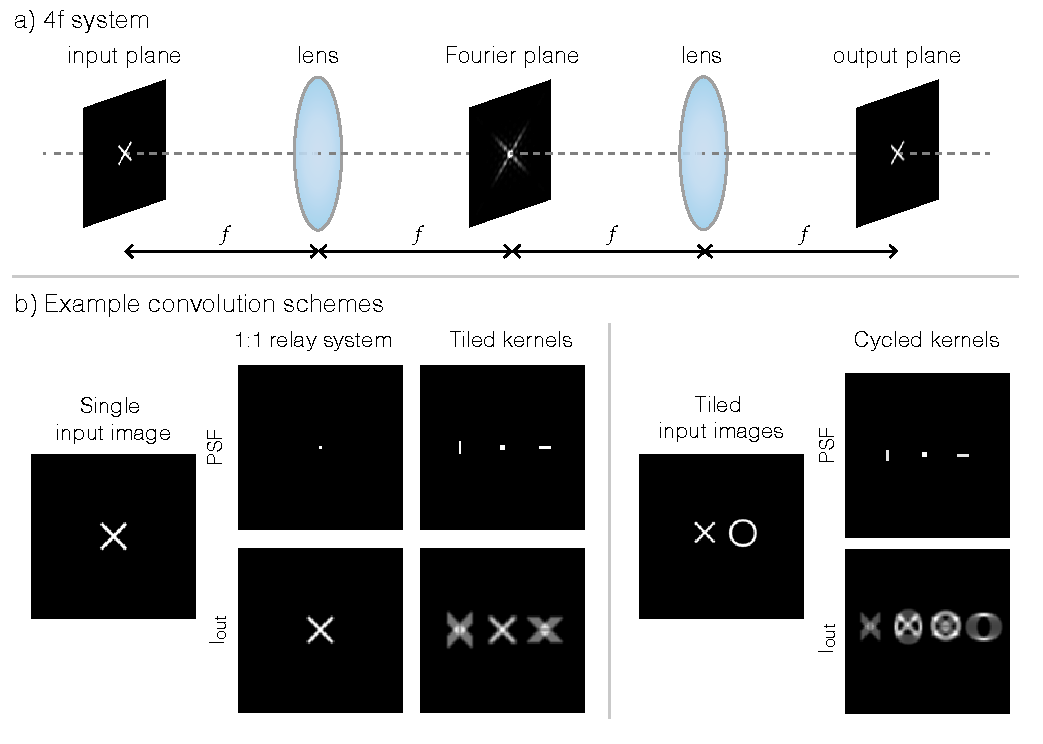
\includegraphics[width=\linewidth]{convolution.pdf}
\caption{Optical convolutional layer}
\label{fig:convolution}
\end{figure}

A CNN typically begins with a convolutional layer, which essentially performs pattern matching with a set of learnable visual filters. A standard convolutional layer takes an input volume of depth $C_\text{in}$, performs a series of correlations with a set of $C_\text{out}$ kernels each with depth $C_\text{in}$, and outputs a new volume of depth $C_\text{out}$. The correlation of the kernel across the width and height of the input volume produces a 2D ``activation map", and stacking the $C_\text{out}$ activation maps for all kernels forms the output volume of depth $C_\text{out}$. Hyperparameters include the spatial extent of the kernel $F$, the stride with which the kernel is applied, and the padding of the input volume. Here we assume a stride of $1$, meaning the kernel is shifted by one pixel at a time, and zero-padding such that the output volume has the same height and width as the input. Each channel of the output image from a single non-strided, zero-padded convolutional layer can be described as:
\begin{equation}
I_\text{out, j}  = \sum_{i = 1}^{C_\text{in}} I_\text{in, i} \ \star \ \text{W}_{i,j}\ , \text{for } j \in 1, 2, \hdots C_\text{out} 
\end{equation}

In linear optical systems, image formation is often modeled as a spatially invariant convolution of the scene with the point spread function (PSF) of the system:
\begin{equation}
I_\text{out}  = I_\text{in} * \text{PSF}
\end{equation}

One way to achieve this setup is with a ``4$f$ system", a basic telescope consisting of two convex lenses performing a cascade of two Fourier transforms (Fig. \ref{fig:convolution}a). The system is so-named due to the placing of the first lens one focal distance, $f$, away from the object plane, producing a Fourier plane another distance $f$ in front of the first lens. The second lens is then placed another distance $f$ from the Fourier plane, producing a conjugate image plane a final distance $4f$ from the original object plane \ref{fig:convolution}. The Fourier plane of such a system can be modulated in amplitude and phase, akin to a bandpass filter in signal processing, which alters the PSF of the system \cite{goodman2008introduction}.  This simple case can be viewed as a convolutional layer with $C_\text{in} = C_\text{out} = 1$ and the flipped PSF as the single kernel. We will also refer to the flipped PSF as the kernel since the flipping is trivial. 

\subsubsection*{Tiled kernels} Now suppose we want $C_\text{out} = n$ where $n >1$. By spatially tiling the multiple kernels as the PSF of the system in an $A \times B$ grid, the output becomes the convolution of the input image with multiple 2D kernels, but now the $n$ outputs are tiled laterally instead of stacked in depth. Consideration can be taken to ensure these outputs are non-overlapping by adjusting the shifts $\Delta x$ and $\Delta y$, if desired. The PSF can be described as
\begin{equation}
{PSF}(x,y) = \sum_{a = 1}^{A}\sum_{b = 1}^{B} W_{aB+b} (x,y) * \delta(x - a\Delta x, y - b\Delta y),
\end{equation}
and the resulting image formation as
\begin{equation}
I_\text{out}(x,y) = [I_\text{in} * PSF](x,y) =\sum_{a = 1}^{A}\sum_{b = 1}^{B}  [I_\text{in} * W_i](x) * \delta(x - a\Delta x, y - b \Delta y)
\end{equation}
where $W$ corresponds to a standard multichannel kernel for a single channel input image. Hence we have a way to convolve a single input image with multiple 2D kernels, with the difference here being that the multiple output channels are tiled across the 2D image plane instead of stacked in a third ``depth" dimension.

\subsubsection*{Cycled kernels}
The next important extension is to incorporate $C_\text{in} = m$ where $m > 1$. If we needed to exactly imitate the digital CNN, we would need $m$ different kernels for each of the $m$ input channels. This could potentially be implemented with many of the single channel modules in parallel, with the addition of a relay that sums $m$ outputs that correspond to the different depth slices of the same kernel, but this type of setup may be prohibitively complicated to build. If we slightly relax our requirements, we could again rely on Fourier optics to perform the summation. Now suppose we have tiled input images in addition to the kernels, simplifying to 1D for now for clarity:
\begin{equation} I_\text{in}(x) = \sum_{j = 1}^m I_j(x)  * \delta(x - j\Delta x),\  PSF(x) = \sum_{i = 1}^m W_i(x)  * \delta(x - i\Delta x)\end{equation}

\begin{align} I_\text{out} &= [I_\text{in} * PSF](x)= \sum_{i=1}^n [I_\text{in} * W_i](x) * \delta(x - i\Delta x)  \\
&= \sum_{i=1}^n \sum_{j=1}^m\left( [I_\text{j} *  W_i](x) * \delta(x - j\Delta x) \right) * \delta(x - i\Delta x) 
\end{align}
This combination of tiled images and tiled kernels results in some cycling of the kernels, but could still potentially offer enough degrees of freedom for certain tasks. Examples of tiled kernels and cycled kernels are shown in Fig. \ref{fig:convolution}b.

\subsubsection*{Large PSFs} Finally, we were curious whether we even needed to think about tiling many small kernels, or rather if we could optimize for one large PSF, and leave it to the optimization to decide whether tiling was the optimal strategy. These approaches are compared in later simulations.

\subsection*{Nonlinear activation layer}
In this paper, we primarily focus on the convolutional layers and apply nonlinear activations in simulations, when they used. However, we review some possible optically addressed approaches for the benefit of further research in this area, which also informs us on what type of activation functions to apply in simulation. 

Nonlinear activation layers are crucial components in the neural network toolbox that allow for modeling of nonlinear relationships between input and output variables. Most commonly used is a rectified linear unit (ReLU), that simply sets all negative values to 0: $\text{ReLU}(x) = \max\{0, x\}$. In an optical intensity-based system, there are no non-negative values, so the standard ReLU function does not directly apply. However, if we consider the purpose of the ReLU layer to zero out some fraction of the neurons below a threshold response level, then we hypothesize that we can accomplish a similar effect by shifting this threshold to a positive value. 

This nonlinear behavior translates to an ideal optical element that is fully opaque when incident light is low intensity and fully transmissive when incident light is above a threshold. A perfectly binary switch is difficult to physically realize, so instead we sought a material that would be less transmissive to lower incident intensities and become more transmissive at higher incident intensities. In fact, this type of nonlinear response is remniscent of the PReLU (parametrized ReLU) \cite{he2015delving} and (Swish) \cite{ramachandran2017searching}, only centered at a positive threshold instead of zero.

Bacteriorhodopsin (BR) is a membrane protein found in the bacterium \textit{Halobacterium salinarium} that has been shown to exhibit logarithmic transmittance at one of its absorbance peaks of $\sim$570 nm \cite{downie1995nonlinear}. The BR protein reversibly cycles between two states with the absorption of light, causing the appearance of a BR film to change from a deep purple to a light transparent purple. Furthermore, the shape of the transmittance function can be tuned by adjusting the concentration and pH of the BR solution before creation of the film \cite{thoma1991bacteriorhodopsin}. Besides BR, visible light-responsive DASA-polymer conjugates have been synthesized that also demonstrate reversible tunable absorption properties dependent on incident light intensity \cite{ulrich2017visible}. This compound shows more of a linear transmittance function, becoming more transparent with higher intensity light \cite{dolinski2017versatile}. We consider these in simulation to assess if a film or gel of these or similar substances could be used as a nonlinear activation layer in an ONN. 

\subsection*{Fully-connected layer}
The fully connected layer is so named because every input neuron is connected to every output neuron.
The output of the previous layer is flattened into a single vector and multiplied with a matrix of size $D_\text{out} \times D_\text{in}$, where $D_\text{in} = H\text{in} \times W\text{in} \times C_\text{in}$. For a limited size of $D_\text{out}$, this elementwise product could be implemented by splitting the input image into $D_\text{out}$ copies and performing an elementwise matrix multiplication using an amplitude mask. Unfortunately, this strategy becomes unreasonable as $D_\text{out}$ grows. 

Fortunately, fully connected layers may not be necessary, as fully convolutional networks have been successful in several prominent cases \cite{lin2013network,iandola2016squeezenet}. For example, if the goal is to classify among $Z$ classes, it is possible to end with a convolutional layer that produces an output with $Z$ channels, and then average each of the $Z$ channels to produce a score for each of the classes. This suggests we may be able to implement a series of optical convolutional layers, divide the final output image into $Z$ subregions, and then take the mean of each of those subregions.

\subsection*{Pooling layer}
Pooling layers can be inserted, commonly between convolutional layers, to reduce spatial size and consequently computation. Pooling operations, for example "maximum", operate on each depth slice independently. One of the main reasons for pooling is to reduce the computing needs by reducing the dimensions of the next input image, which we do not need to consider in an optical system. Otherwise, pooling may improve training and prevent overfitting.

While it is not obvious how to take the spatial maximum of an optical signal without active sensing, average pooling can be approximated with a reduction in the spatial resolution of the image. This can be accomplished with a low-pass filter, i.e. a small iris placed in the pupil plane of the last $4f$ system. Spectral pooling is another interesting concept used in spectral representations of CNNs that carries over easily to our ONN setup \cite{rippel2015spectral}. Spectral pooling can be viewed as a generalization of low-pass filter pooling, in particular allowing for specific bandwidths to be selected for using custom amplitude masks. We only mention pooling layers here but do not explore these in our further experiments, as they were not essential for our analysis of convolutional layers.



\section{Learning an Optical CNN}
\label{sec:simulation}
\red{This may be moved to Methods.}

To train our optical CNNs, we build the forward model of computational light transport in a Tensorflow framework and use built-in backpropagation and stochastic gradient-based optimizers to learn the weights, both of the PSFs and the optical elements.

\subsection*{Spatial domain optimization}
Our strategy to building understanding of optical CNNs was to begin with a vanilla CNN and incrementally add constraints and features unique to optical models. Hence we begin in the spatial domain, assuming there exist optical elements that can produce the PSFs found by the optimization. From a standard CNN, we remove biases, impose non-negativity on the input and weights, and reduce the number of channels of the kernels while increasing their height and width. We also substitute our own nonlinearities for the standard ReLU function. Since some of the PSFs we try to optimize are much larger than normal, we use an FFT-based convolution to increase speed. 

\subsection*{Phase mask optimization}
After spatial domain optimization, the task still remains of connecting these desired PSFs to an optical implementation. As mentioned earlier, the Fourier plane of a $4-f$ system can be modulated with an aperture transfer function (ATF) to control the incoherent PSF of the optical relay:
\begin{equation} PSF(x,y) = |\mathcal{F}\{ATF(k_x, k_y)\}(x,y)|^2,\end{equation}
where $ k_x = \frac{x}{\lambda f}$ and $k_y = \frac{y}{\lambda f}$ denote spatial frequencies and $\lambda$ is the wavelength of light. 
The ATF is a potentially complex function that can be decomposed into amplitude and phase as $ATF = A(k_x, k_y)\cdot \exp(i \Delta \phi (k_x, k_y))$, where local amplitude $A$ can be implemented with a (usually binary) transparency mask, and phase shifts $\Delta \phi$ can be realized with a clear optical element of spatially varying thickness, which controls the optical path length and thereby phase shift induced by the element. To prevent loss of light and reduce the fabrication complexity of the ATF-defining optical element, we restrict our optimization to phase-only control. 

Given the optimized PSF(s) from the spatial domain optimization, we now want to optimize phase masks that can generate these desired PSFs:
\begin{equation} \underset{\phi}{\text{minimize}} \|PSF_\text{opt} - |\mathcal{F}\{e^{i\Delta \phi}\}|^2\|^2_\text{F}
\end{equation}
where $\|\cdot\|_\text{F}$ denotes the Frobenius norm.  Many different approaches have been taken to solve the phase retrieval problem \cite{shechtman2015phase}, but since we are already using a learning-based approach above, we can use the Tensorflow framework here as well. We initialize a random phase mask and propagate training images through the current iterate of the $4f$ system. An error is calculted against the ground truth images where the training images are convolved with the desired $PSF_\text{opt}$, and then the gradients are backpropagated to the phase masks. 

\subsection*{End-to-end optimization}
Instead of separately optimizing the PSFs and then the corresponding phase masks,  we also explored the possibility of an end-to-end optimization. To combine these steps into a single optimization problem, we implement a variant of the classification Tensorflow model where the phase mask heights were the optimizable parameter rather than the PSF weights themselves, such that the gradients of the classification error function are backpropagated all the way to the phase mask heights. Unfortunately, this approach did not always produce desired results, as we will show in the next section. 

\section{Evaluation of Optical CNNs}
\label{sec:simulations}
We use simulations to better understand the performance of optical CNNs. \\
\red{Fig. 2}: diagram of possible ONN models.
\red{Table 1:} Results.
 Introduce toy classification problem(s?), discuss constraints.

\subsection{Learned Optical Correlator}
For our first experiment, we simulated a system with a single optical convolutional layer to confirm that our proposed optical convolution layer would function as expected. A single convolutional layer is essentially an optical correlator.  

Here we are able to use end-to-end learning. \\


\red{Possible figure with learned phase mask and PSF.}

While this was interesting, optical correlator is not powerful enough for more difficult classification tasks, for example with natural images or with more categories. Also, with a single layer, it was not necessarily a CNN.

\subsection{Hybrid optoelectronic CNN} 
Next we keep one optical convolutional layer but add on more after. 
\red{Fig. 3: Hybrid ONN phase masks and PSFs.}
	Grayscale \\

\subsubsection{Pseudo-negative weights}
	Talk about the dual channel positive and negative weights\\


\subsubsection{Color filters - Vincent}



\subsection{Fully optical CNN} 
Doesn’t fully work, but can discuss some results

\section{Optical Prototype}
\label{sec:prototype}
Implement the hybrid optoelectronic two-layer neural network. Goal is to show that the hybrid ONN can perform on par with the electronic ONN, with the same number of layers, and better than the electronic ONN with one fewer layer.\\
\begin{figure}
\centering
\includegraphics[width=10cm]{prototype.jpg}
\caption{Optical prototype}
\label{fig:prototype}
\end{figure}
\red{Table. 2: results}

\section{Discussion}
\label{sec:discussion}
\begin{itemize}
\item Not straightforward to generalize first optical conv. layer to multiple optical layers
\item Discuss importance of negative weights – \red{Vincent?}
\item Instead of trying to replicate a CNN exactly, could take advantage of optical transformations that aren't as practical in computations. For example, we use a 4f system for convolution, but this requires two extra lenses. Perhaps a single custom learned optical element can be used instead.
\item In the future, exploit other properties of light (polarization, phase)	
\item Specifically, coherent light and holography, photonics
\end{itemize}

\section{Conclusion, p. 14}
\label{sec:conclusion}
We hope this will inspire more research in the area. 

\clearpage

\bibliographystyle{splncs}
\bibliography{../bibliography}
\end{document}
